
%Copyright (C) 2016 by Krishneel@JSK Lab, The University of Tokyo

\documentclass{standalone}
\begin{document}

\subsection{Hardwares}

We developed the uav with hex rotors as shown in Fig.\ref{fig:task1-uav}. As descrbied in  Fig.\ref{fig:task1-uav-platform}, this aerial robot consists of onboard sensors such as IMU, barometer, laser sensor, GPS for basis hovering flight control, as well as the original flight controller and high level processor. The monocular camera is installed for the further egomotion estimation. The total weight of the uav is 4.3Kg, while the flight time can reach 20min with heavy vision processing on the onboard processor. We have achieved the outdoor flight with autonomous altitude hold mode using our original sensor fusion algorithm(Fig.\ref{fig:task1-outdoor-flight}).

\begin{figure}[h]
  \begin{center}
    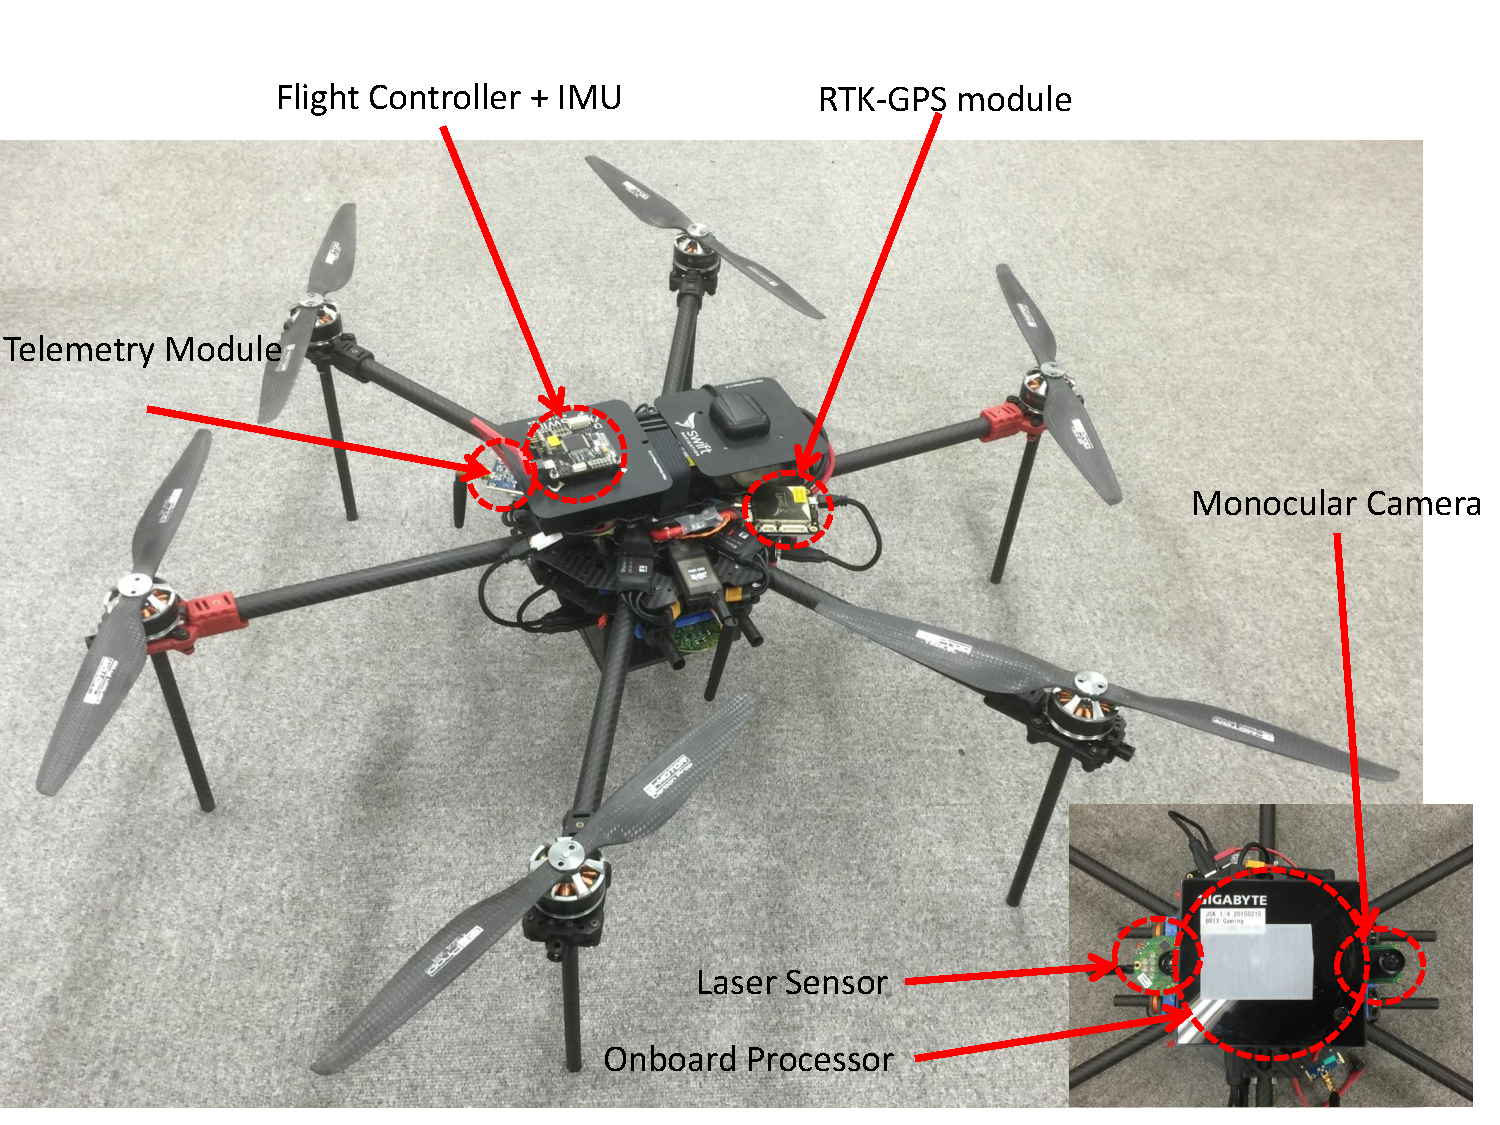
\includegraphics[clip,  bb=0 0 710 502,  width=\columnwidth]{sections/task1/images/task1-tarrot680.pdf}
    \caption{Image of task1 UAV(Hawk)}
    \label{fig:task1-uav}
  \end{center}
\end{figure} 

\begin{figure}[h]
  \begin{center}
    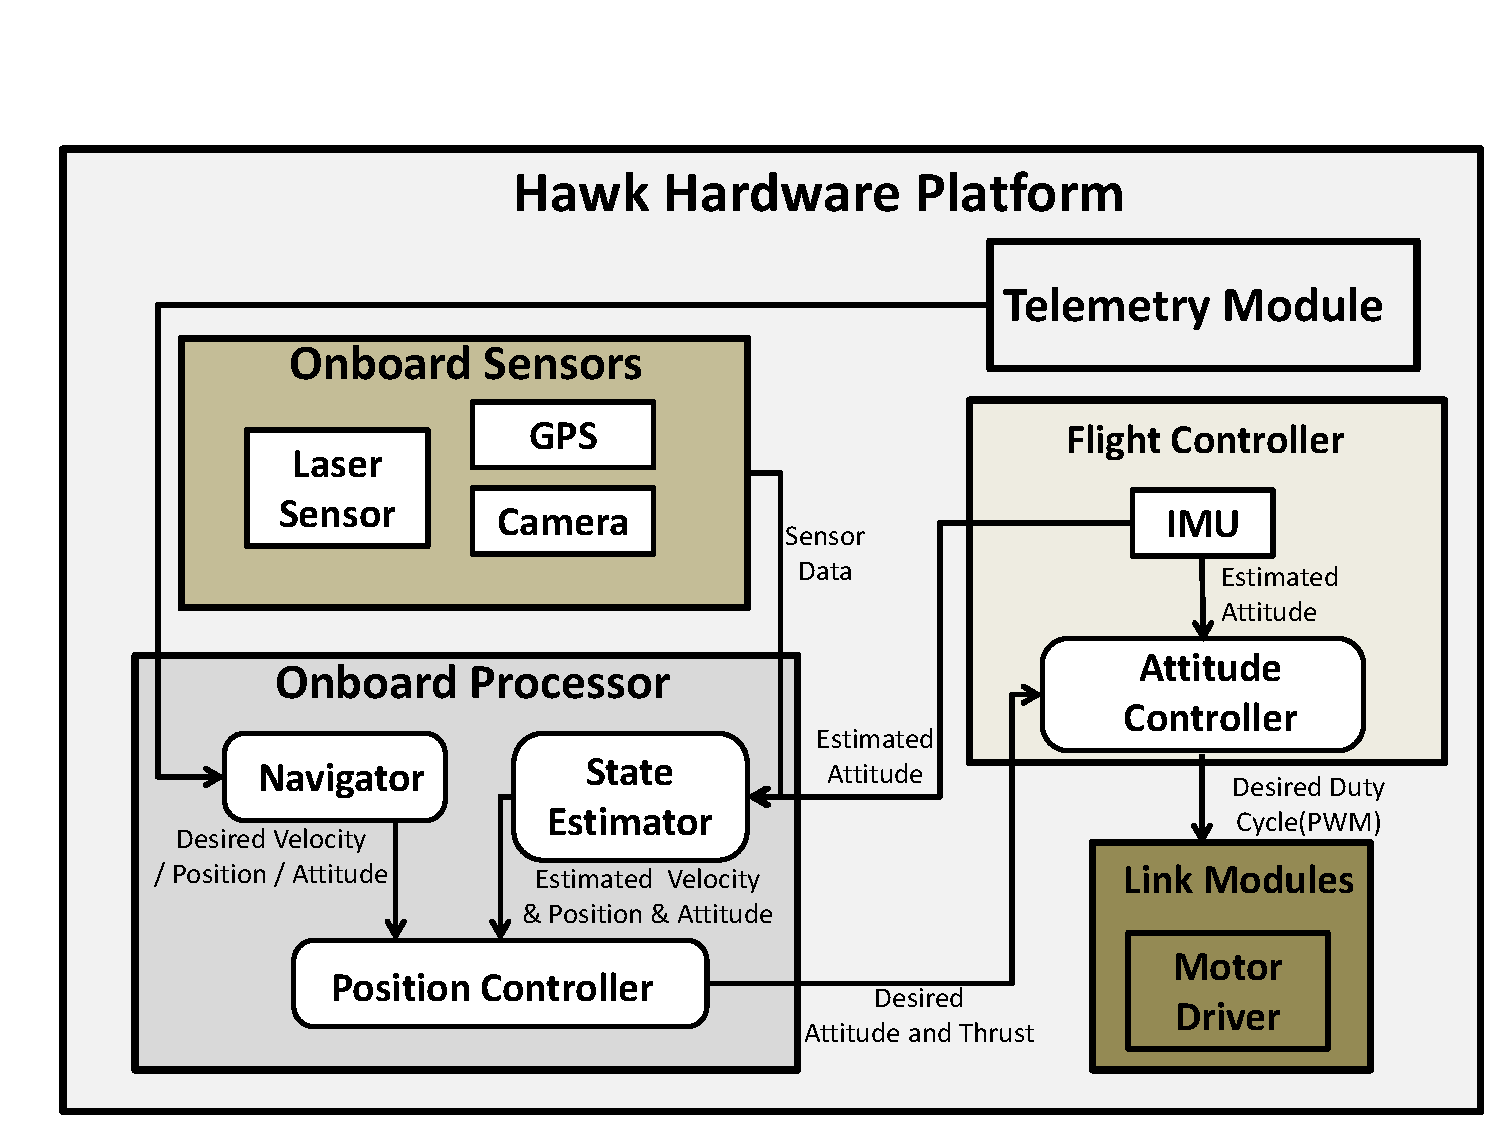
\includegraphics[clip,  bb=0 0 720 500,  width=\columnwidth]{sections/task1/images/hawk-platform.pdf}
    \caption{Hardware platform of "Hawk"}
    \label{fig:task1-uav-platform}
  \end{center}
\end{figure} 

\begin{figure}[h]
  \begin{center}
    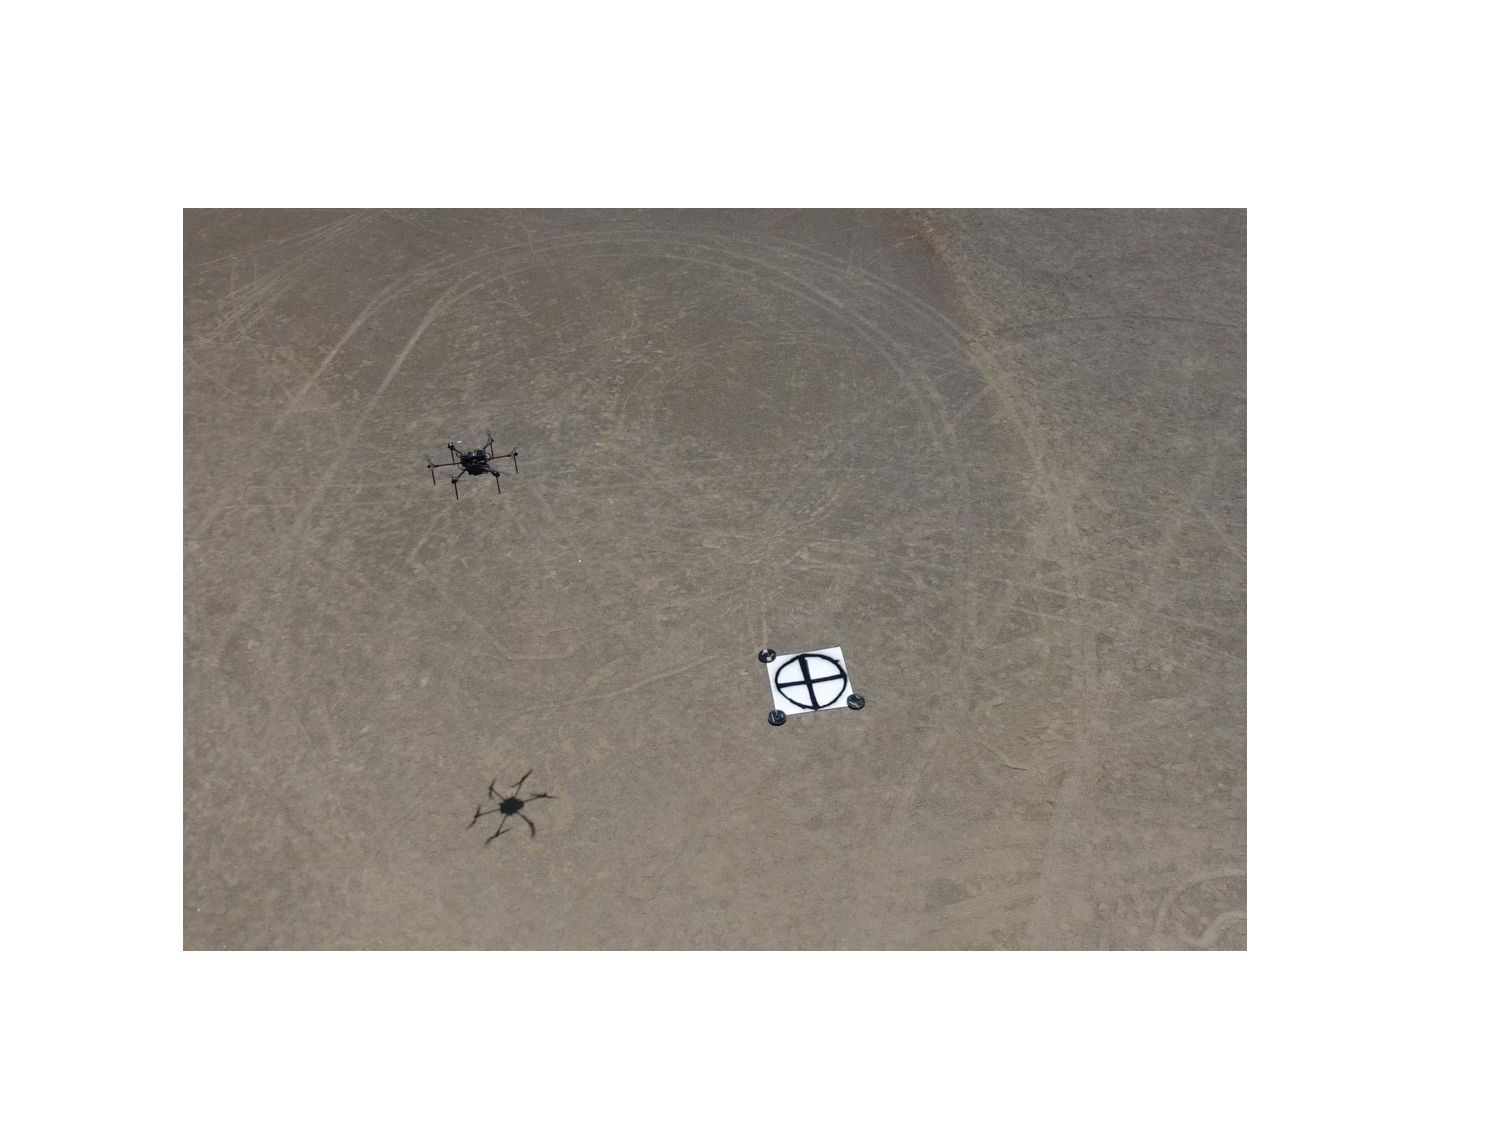
\includegraphics[clip,  bb=88 84 599 440,  width=\columnwidth]{sections/task1/images/task1-outdoor.pdf}
    \caption{Image of outdoor flight }
    \label{fig:task1-outdoor-flight}
  \end{center}
\end{figure} 



\end{document}
